\section{Preliminaries}\label{sec:prelim}


In this section, we introduce concepts that we are going to use in future sections. We start by defining datalog, which we will formalize later. After that, we review the concept of certifying algorithms and finally, we introduce Lean.


\subsection{Datalog}
Datalog is a logic programming language and can be syntactically considered as a subset of Prolog. An introduction to datalog and other query languages can be found in \cite{alice}, which we recall next. Some knowledge about first-order logic may be beneficial, which be found for example in \cite{logic}.

In order to write datalog rules, we require the existence of three at most countable sets $V, C$ and $P$, where $V$ represents variables, $C$ represents constants and $P$ represents predicate symbols. Every predicate symbol $p$ in $P$ has an arity $ar(p) \in \mathbb{N}$, where $0 \in \mathbb{N}$.

\begin{example}
    In general, we consider in this work $R$ as strings that start with a capital letter, $V$ as strings that start with a question mark and $C$ as all other non-empty strings.
\end{example}

\begin{example}
In a more concrete example we have the variables $V= \{?x,?y,?z\}$ and constants $C= {1,...,7}$. The predicate symbols are the binary predicates (i.e. they have an arity of two) $R$ and $E$ and the nullary (i.e. arity zero) predicate $Q$.
\end{example}

In the language of first-order logic as in \cite{logic}, $C$ and $P$ build the signature of the language we are going to build. We note that this fragment of first-order logic does not use function terms.

The following definitions are adapted from logic for the signature above.

A \textit{term} is either a variable or a constant. In order to differentiate meaningfully between them, we require that $C \cap V = \empty$ so that no symbol is both a variable and a constant. As long as both $C$ and $V$ are finite, we will only have a finite amount of terms. This is in contrast to general first-order logic or logic programming where function symbols can lead to an infinite amount of terms even if the signature is finite.

\begin{contexample}
    Examples of terms in our language are $?z$, $2$, $5$ or $?x$.

    A counterexample would be $word$ or $A$ as those elements do not occur in either $C$ or $V$.
\end{contexample}

An \textit{atom} is an expression of the form $A(t_1,...,t_n)$ for $n \in \mathbb{N}$ where $A$ is a predicate symbol ($A \in P$) and $t_1,..,t_n$ are terms. Additionally, we require that $n$ is the arity of $A$, i.e. $ar(A) = n$.

\begin{contexample}
    Examples for atoms are here: $Q(), R(?x,?y), E(2,3)$ or $E(?x, 7)$. In every atom, the number of terms matches the arity of the predicate symbol. We note that it is allowed to mix variables and constants in the terms of an atom.

    A first counterexample would be $Q(a)$ because the arity does not match. 
    Another counterexample would be $R(E(2,3),4)$ because $ E(2,3)$ is not a term.
\end{contexample}

In the example, some atoms used only constants in their terms, while others included variables. This is expressed by $Vars(A(t_1,...,t_n)) = \{t_i \mid t_i \in C\}$. If for some atom $a$ $Vars(a)$ is empty, we call this a \textit{ground atom}.

\begin{contexample}
    In the previous example $Q()$ and $E(2,3)$ are ground atoms. The first does not have any terms at all, whereas the other only uses constants.

    For the other atoms we have $Vars(R(?x,?y)) = \{?x,?y\}$ and $Vars(E(?x, 7)) = \{?x\}$, so that they are not ground atoms.
\end{contexample}

A \textit{rule} is an expression of the form $H \leftarrow B_1 \and ... B_n$ for atoms $H$ and $B_i$ for $n \in \mathbb{N}$. We call $H$ the \textit{head} of the rule and $B_1,..., B_n$ the \textit{body} of the rule and define the functions $head(r) = H$ and $body(r) = {B_i}$. We allow rules with an empty body. These rules are called \textit{facts}.

We can generalize the $Vars$ function to rules and use this to define \textit{ground rules}. For a rule $r = H \leftarrow B_1 \and ... B_n$, we define \[Vars(r) = Vars(H) \cup \bigcup_{i \in \{1,..., n\}} Vars(B_i)\] and call $r$ a ground rule if $Vars(r) = \emptyset$. This means that a rule is a ground rule if the head and every atom in the body is a ground atom.

\begin{contexample}
    Examples for rules are $E(1,2) \leftarrow $, $Q() \leftarrow E(?x,?y)$ or $T(?x,?z) :-E(?x, ?y), T(?y,?z)$.

    $E(1,2) \leftarrow $ is both a fact and a ground rule, but not every fact is a ground rule as for example $E(?x, ?x) \leftarrow$
\end{contexample}

A \textit{program} $P$ is a finite set of rules. We only consider finite sets as infinite sets are difficult to express in practice.

\begin{contexample}
    We consider the program $P = \{$

    \begin{equation}
    \begin{split}
    E(1,2) &\leftarrow \\ E(1,3) &\leftarrow \\ E(3,5) &\leftarrow \\ E(4,6) &\leftarrow \\E(4,7) &\leftarrow\\ Q() &\leftarrow \\ T(?x,?y) &\leftarrow E(?x,?y) \\ T(?x,?x) &\leftarrow \\ T(?x, ?z) &\leftarrow T(?x,?y) \and T(?y, ?z)
    \end{split}
    \end{equation}
    $\}$, which contains both facts and other rules.
\end{contexample}

With this, we have introduced all the needed elements for the syntax of datalog, but we have not yet spoken of the semantics of datalog. What is the program $P$ supposed to express?

We have noted the similarities between datalog and first-order logic when defining the syntax of datalog. Nonetheless, neither rules nor programs are direct elements of first-order logic. It is however not difficult to bring them into a form, where we can interpret them as elements of first-order logic and use the semantics of first-order logic for it.

The symbol $\leftarrow$ used in the definition of rules appears to be very similar to the implication $\rightarrow$ from first-order logic so we can use this fact to transform any rule into a first-order formula. This formula has still free variables so that we universally quantify over all remaining variables to gain a sentence. After doing this we can consider any program as a finite first-order theory.

\begin{contexample}
    The equivalent sentence for the fact $E(1,2) \leftarrow$ is 
    
    \[E(1,2)\]
    
    
    and for the rule $T(?x, ?z) \leftarrow T(?x,?y) \and T(?y, ?z)$ is 
    
    \[\forall ?x,?y,?z. T(?x,?y) \land T(?y, ?z) \rightarrow T(?x, ?z)\]
\end{contexample}

The semantics of a first-order theory or sentence are its models. Unfortunately, a theory may have multiple models as the following example shows for the theory for $P$.


\begin{contexample}
    Any fact must be true in a model, but the implications allow us more freedom. As both $E$ and $T$ are binary predicates, we can represent them as a graph. We use blue, when both $E$ and $T$ are present, green for only $T$ and orange for $E$

    \begin{figure}
        \centering
        \begin{minipage}[b]{0.45\linewidth}
        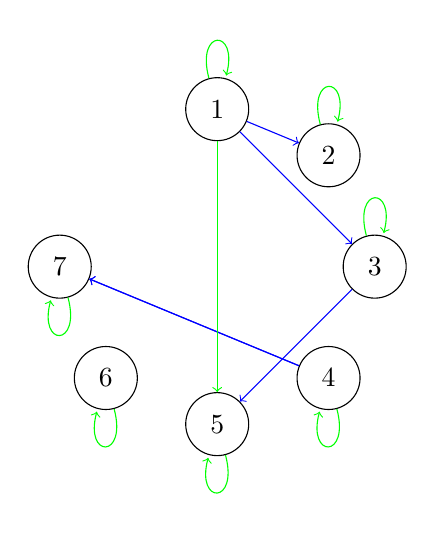
\begin{tikzpicture}[, every node/.style={circle, draw, minimum size=8mm}]
            % Nodes
            \node (1) at (90:2) {1};
            \node (2) at (45:2) {2};
            \node (3) at (0:2) {3};
            \node (4) at (-45:2) {4};
            \node (5) at (-90:2) {5};
            \node (6) at (-135:2) {6};
            \node (7) at (180:2) {7};

            %self loop
            \foreach \i in {1,...,3} {
                \draw[->,green] (\i) edge [loop above] (\i);
            }
            \foreach \i in {4,...,7} {
                \draw[->,green] (\i) edge [loop below] (\i);
            }

            % Edges
            \draw[->,blue] (1) -- (2);
            \draw[->,blue] (1) -- (3);
            \draw[->,blue] (3) -- (5);
            \draw[->,blue] (4) -- (7);
            \draw[->,blue] (4) -- (7);
            \draw[->,green] (1) -- (5);
        \end{tikzpicture}
        \caption{First model}
    \end{minipage}
    \quad
    \begin{minipage}[b]{0.45\linewidth}
        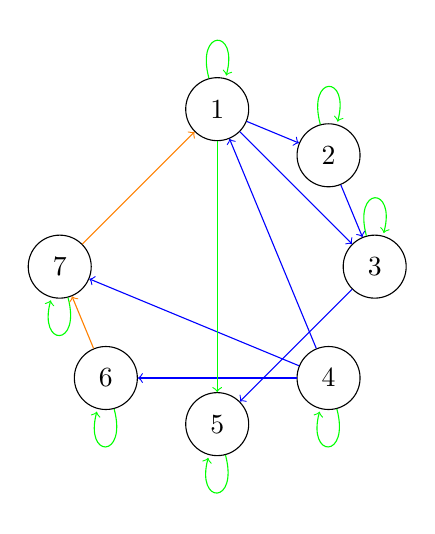
\begin{tikzpicture}[, every node/.style={circle, draw, minimum size=8mm}]
            % Nodes
            \node (1) at (90:2) {1};
            \node (2) at (45:2) {2};
            \node (3) at (0:2) {3};
            \node (4) at (-45:2) {4};
            \node (5) at (-90:2) {5};
            \node (6) at (-135:2) {6};
            \node (7) at (180:2) {7};

            %self loop
            \foreach \i in {1,...,3} {
                \draw[->,green] (\i) edge [loop above] (\i);
            }
            \foreach \i in {4,...,7} {
                \draw[->,green] (\i) edge [loop below] (\i);
            }

            % Edges
            \draw[->,blue] (1) -- (2);
            \draw[->,blue] (1) -- (3);
            \draw[->,blue] (3) -- (5);
            \draw[->,blue] (4) -- (6);
            \draw[->,blue] (4) -- (7);
            \draw[->,blue] (2) -- (3);
            \draw[->,green] (1) -- (5);
            \draw[->, orange] (6) -- (7);
            \draw[->, orange] (7) -- (1);
            \draw[->,blue] (4) -- (1);
        \end{tikzpicture}
        \caption{Second model}
    \end{minipage}
    \end{figure}
    
    The first model expresses $T$ as the reflexive transitive closure of the input $E$, whereas the second model expands the first model and adds more additional atoms to a model.
\end{contexample}

Such an ambiguity is not ideal when we want to compute the query results of datalog. Some fragments of logic programming allow multiple models such as answer-set programming, but for datalog, we want a unique model. This is known as the least model. For this, we need to define what least means and show that it exists.

We call a set of ground atoms an \textit{interpretation}. An interpretation represents all true atoms. We want to define the model property from first-order logic for this definition and show then that there exists a least model according to the subset relation.

Recall from first-order logic that $\forall x. \phi(x)$ holds in a structure $\mathcal{A}$ if any element $a \in \mathcal{A}$ we have that $\phi(a)$ holds. As we do not have any function symbols all elements in the universe are constants, so instead of using the universal quantifier we could just create rules by replacing variables with all possible constants.
Formally, this is defined using \textit{groundings} or \textit{instantions} which are functions that map variables to constants. We can apply a grounding $g$ to an atom by replacing every variable $v$ in the terms by $g(v)$ and apply $g$ to a rule by applying it to the head and every atom in the body. At the end of this, we have replaced every variable by a constant and have gained a ground rule. 
The ground program $ground(P)$ of a program $P$ is the set of all ground rules that are the result of applying some grounding to a rule from $P$

We call a ground rule $r$ \textit{true} in an interpretation $I$ if whenever $Body(r)$ is a subset of $I$, then also $Head(r)$ is in $I$.  We call an interpretation $I$ a \textit{model} of a program $P$ if every rule of $ground(P)$ is true in $I$.

So now we have defined models and can define the least model as well. We still need to show that the least model exists for which the following lemma is helpful.

\begin{fact}\label{fact:ModelIntersection}
Let $M_1, M_2$ be two models of a program $P$. Then also $M_1 \cap M_2$ is a model of $P$.
\end{fact}

Therefore the intersection of all models is a model as well and due to the properties of the intersection it is least according to the subset relation. 

In total, we call \[\bigcap_{\text{$M$ is model of $P$}} M\] the \textit{least model} of $P$ and refer to this characterization as the \textit{model-theoretic semantics} of $P$.

\begin{contexample}
    In this example, the first model is actually the least model and the second model is just some other model.

    Therefore the semantic of this program is whenever $Q()$ is given, the reflexive-transitive closure of $E$. 
    If $Q()$ is not given then it is only the reflexive closure.

    Additionally, we see that the rules for $T$ encode general rules whereas the other rules are more a specific input. We might want to reuse these rules for many different instances of $E$, but so far we also need to write a new program.
\end{contexample}

The example raises questions about the reusability of a program. Additionally, we talked in the introduction about database queries but never talked about databases. 

We consider a \textit{database} as a set of ground atoms similar to an interpretation. What is now the semantics of a program $P$ and a database $d$? We simply add every element of $d$ as a fact to $P$ and reuse the previous semantics. Additionally, we can also move all the specific facts from the program into the database and gain a reusable program.
An alternative model definition for a pair of $P$ and $d$ is therefore: An interpretation $I$ is a model for $P$ and $d$ if every ground atom from $d$ is in $I$ and every rule from $ground(P)$ is true in $I$. \cref{fact:ModelIntersection} holds again and we reuse the definition for the database and program case.

Both views are equivalent. We have shown how we can simulate a database by a program. We can simulate the program case with the program and database case by simply using an empty database.

We have now defined the semantics and shown a connection with databases. But this definition is not exactly ideal. In order to find the semantics of a program we would need to check all interpretations and then intersect them all. This is computationally expensive. Is there a simpler way?

We can define a function that computes the least model in a more direct way. For this, we consider the case where only the program $P$ is present.

Consider an interpretation $I$. We call a ground atom $a$ an \textit{immediate consequence} of $I$ if there exists a ground rule $r$ in $ground(P)$ with the head $a$ and $Body(r) \subseteq I$.

The immediate consequence operator $T_P$ adds all immediate consequences to a model. 

\[T_P(I) = \{ a \mid \text {$a$ is an immediate consequence of $I$}\} \]

A fixed point of a function $f$ is an element $k$ such that $f(k) = k$. The repeated application of $T_P$ starting from $\emptyset$ yields a fixed point that is equal to the model-theoretic semantics of a program $P$. 

\begin{contexample}
    We consider again the program $P$. 

    Due to the fact $E(1,3) \leftarrow$, $E(1,3)$ is an immediate consequence of $\emptyset$. Applying $T_P$ again, we have that $T(1,3)$ is an immediate consequence of $\{E(1,3)\}$ due to the rule $T(?x,?y) \leftarrow E(?x, ?y)$ with the grounding 
    
    \[
    g(v) =
    \begin{cases}
        1 & \text{if } v = ?x \\
        3 & \text{else}
    \end{cases}
    \]

    Applying this to every fact, we gain an interpretation $I$ that contains $T(1,3)$ and $T(3,5)$. Then $T(1,5)$ is an immediate consequence of $I$ due to the rule $T(?x, ?z) \leftarrow T(?x,?y) \and T(?y, ?z)$ and the grounding 

    \[
    g'(v) =
    \begin{cases}
        1 & \text{if } v = ?x \\
        3 & \text{if} v = ?y \\
        5 & \text{else}
    \end{cases}
    \]
\end{contexample}

The least fixed-point of $T_P$ is called the \textit{fixed-point semantics} of $P$ and is the basis for most implementations of datalog reasoners. 

Our goal is to explain why an atom is in the datalog result. The third important semantic of datalog helps here. 

A tree $t$ of ground atoms is a proof tree for a ground atom $a$ in a program $P$ and database $d$ if the following three conditions hold:

\begin{enumerate}
    \item the root of $t$ is $a$
    \item for every node $n$ and its children $l$ in $t$ one of the following two conditions holds: 
    \begin{enumerate}
        \item $n \leftarrow l_1 \land ... l_n$ for $l_1,.., l_n \in l$ is a ground rule from $ground(P)$, or
        \item $n$ is a leaf and $n$ is in the database.
    \end{enumerate}
\end{enumerate}

\begin{figure}
    \centering
    \begin{subfigure}[b]{0.45\linewidth}
    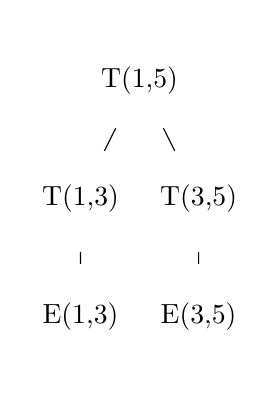
\begin{tikzpicture}[, every node/.style={circle}]
        \node {T(1,5)}
            child {node {T(1,3)}
                child {node {E(1,3)}}
                }
            child {node {T(3,5)}
                child {node {E(3,5)}}};
    \end{tikzpicture}
    \label{prelim:validTree}
    \caption{A valid proof tree}
    \end{subfigure}
    \quad
    \begin{subfigure}[b]{0.45\linewidth}
        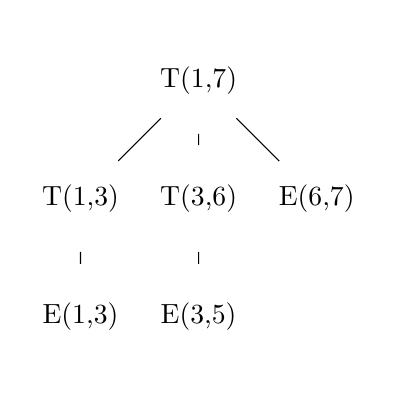
\begin{tikzpicture}[, every node/.style={circle}]
            \node {T(1,7)}
                child {node {T(1,3)}
                    child {node {E(1,3)}}
                    }
                child {node {T(3,6)}
                    child {node {E(3,5)}}}
                child {node {E(6,7)}};
        \end{tikzpicture}
        \caption{An invalid tree}
        \label{prelim:invalidTree}
    \end{subfigure}
    \end{figure}

\begin{contexample}
    The tree in \cref{prelim:validTree} is valid. The leaves of this tree are facts and all other nodes represent ground rules from $ground(P)$ in the previous step.

    The tree in \cref{prelim:invalidTree} is not valid. $E(6,7)$ is neither a fact nor in the database. Additionally there is no rule in $P$ that can result into $T(1,7) \leftarrow T(1,3) \land T(3,6) \land E(6,7)$.
\end{contexample}

The proof-theoretic semantics of a program $P$ and database $d$ is the set of ground atoms that have a valid proof tree. Again this can be shown to be equal to the other semantic definitions. We will formally prove the equality of the proof-theoretic and the model-theoretic semantics of datalog in this work.

In the rules of the program $P$ we note a special rule of the form $T(?x, ?x) \leftarrow$. It is a fact, but not a ground rule and the only rule where this is the case. 
We call a rule $H \leftarrow B_1 \land ... \land B_n$ \textit{safe}, if every variable that occurs in the head also occurs in the body, i.e. \[Vars(H) \subseteq \bigcup_{i \in \{1,..,n\} } Vars(B_i) \]

We call a program safe if every rule in the program is safe. Safe programs are considered better because their result does not depend on the set of constants $C$ which is in practice often either not given or infinite, but only on the specific database and/or the facts in the program.

\begin{contexample}
    We can transform $P$ into the safe program $P'$ by adding a new unary predicate $N$ to the predicate symbols. $P'$ is then the union of $P \setminus \{T(?x, ?x) \leftarrow \}$ and the following rules:
    \begin{equation}
        \begin{split}
            N(?x) &\leftarrow E(?x, ?y) \\
            N(?y) &\leftarrow E(?x, ?y) \\
            T(?x,?x) &\leftarrow N(?x) \\
        \end{split}
    \end{equation}

    The new predicate $N$ (for nodes) represents any elements that occur in the $E$ relation and is used in the body for the reflexive rule.

    If some constants are desired that do not occur in any $E$ relation, one can also directly encode that into the database.
\end{contexample}

What are the semantics of this newly created safe program $P'$? It turns out, that it is equal to the semantics for $P$ for all original predicates, i.e. if we remove all ground atoms that use $N$ we gain the same result. Therefore we state that any program can be transformed into an equivalent safe program.

\subsection{Certifying algorithms}

\begin{figure}
    \centering
    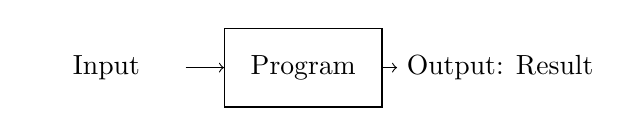
\begin{tikzpicture}[node distance=2.5cm and 20cm, auto]

        \tikzstyle{block} = [rectangle, minimum width=2cm, minimum height=1cm, text centered]
        
        \node [block] (box1) {Input};
        \node [block, right of=box1, draw] (box2) {Program};
        \node [block, right of=box2] (box3) {Output: Result};
        
        \draw [->] (box1.east) -- (box2.west);
        \draw [->] (box2.east) -- (box3.west);
        
    \end{tikzpicture}
    \caption{A convential algorithm}
    \label{fig:programNormal}
\end{figure}

\begin{figure}
    \centering
    \begin{tikzpicture}[node distance=3cm and 3cm, auto]

        \tikzstyle{block} = [rectangle, minimum width=2cm, minimum height=1cm, text centered]
        
        \node [block] (box1) {Input};
        \node [block, right of=box1, draw] (box2) {algorithm};
        \node [block, below of=box3] (box4) {Certificate};
        \node [block, right of=box2] (box3) {Result};
        \node [block, right of=box3, draw ] (box5) {Checker};
        \node [block, right of=box5 ] (box6) {Accept/Not accept};
        \node [block, above of= box6] (box7) {Output};

        \draw [->] (box1.east) -- (box2.west);
        \draw [->] (box2.south) |- (box4.west);
        \draw [->] (box2.east) -- (box3.west);
        \draw [->] (box3.east) -- (box5.west);
        \draw [->] (box4.east) -| (box5.south);
        \draw [->] (box5.east) -- (box6.west); 
        \draw [->] (box3.north) |- (box7.west); 
    \end{tikzpicture}
    \caption{A certifying algorithm algorithm}
    \label{fig:certifyingAlgorithm}
\end{figure}

Most algorithms one encounters either in books like \cite{AlgorithmsBook} or in real programs are comparable to \cref{fig:programNormal}. We have an input, give this into an algorithm which is a black box for us and then we receive a result as an output. Without inspecting the implementation we have to trust that the results are correct.
An alternative to this are \textit{Certifying algorithms} depicted in \cref{fig:certifyingAlgorithm}. They offer an explanation in addition to the result that can be checked independently by the checker or the user themselves. We follow the presentation in \cite{CertAlg} which offers information far beyond this section as well. 

Recall a definition of the class NP from complexity theory:

\begin{definition}[\cite{complexityBook}]
    A language $L \subseteq \{0,1\}^\star$ is in NP if there exists a polynomial $p: \mathbb{N} \to \mathbb{N}$ and a polynomial-time Turing machine $M$ such that forall $x \in \{0,1\}^\star$:

    \[ x \in L  \Leftrightarrow \exists u \in \{0,1\}^{p(|x|)}\text{ s.t. } M(x,u) = 1\]

    If $x \in L$ and $u \in \{0,1\}^{p(|x|)}$ satisfy $M(x,u) = 1$, then we call $u$ a certificate for $x$
\end{definition}

We can generalize this and require an algorithm not only to give us an output $x$ but also a certificate $u$ as a reason why $x$ is the correct output. Then we can either check by ourselves that $x$ is a correct solution according to $u$ or use another program that checks this. As verifying a solution is never harder than computing it, the checker is usually simpler so that we either see directly that the checker is correct or we can formally verify it.

The formal framework of \cite{CertAlg} defines certifying algorithms in the following way. We consider the set $X$ of input values and the set $Y$ of output values of a function $f$. A predicate $\phi: X \to \{true, false\}$ states a precondition for the inputs and another predicate the postcondition $\psi: X \times Y \to \{true, false\}$, $\phi$ allows us the algorithm to only accept part of the input space and $\psi(x,y)$ typically expresses that $y$ is a valid output for the input $x$. In cases where $x$ is not a valid input, we use the new symbol $\bot$ to denote that the algorithm does not return anything and denote by $Y^\bot = Y \cup \{\bot\}$.
The certificate or \textit{witness} from a set $W$ and its correctness is expressed by the predicate $\mathcal{W}: X \times Y^\bot \times W$ with the following properties:

\begin{enumerate}
    \item \textbf{Strong witness property}: Consider a triple $(x,y,w)$ that satisfies the witness predicate $\mathcal{W}$. If $y=\bot$, i.e. the input is not valid, we want $w$ to be a proof of this fact. Else we have that $y\in Y$ and we want $w$ to be a proof that the postcondition is satisfied, i.e.
    \[ \forall x,y,w (y = \bot \land \mathcal{W}(x,y,z) \rightarrow \neg \phi(x)) \land (y \in Y \land \mathcal{W}(x,y,z) \rightarrow \psi(x,y)) \]
    \item \textbf{Simplicity}: This statement above has a simple proof
    \item \textbf{Checkability}: It is possible to check efficiently if $\mathcal{W}(x,y,z)$ holds for a triple $(x,y,z)$
\end{enumerate}

A \textit{(strongly) certifying algorithm} is an algorithm that stops on all inputs $x \in X$ and returns a tuple $\langle y, w\rangle$ such that $\mathcal{W}(x,y,w)$ holds.

This is explained in the following examples. We start with an example from graph theory.

\begin{example}[\cite{CertAlg}]
    Consider the problem of deciding whether a graph $G=(V;E)$ is bipartite, i.e. there exists a partition of $V$ into $V_1, V_2$ with $V = V_1 \cup V_2$ and $V_1 \cap V_2 = \emptyset$, such that for all edges $e \in E$ we have that $e \cap V_1 \neq \emptyset$ and $e \cap V_2 \neq \emptyset$, so that all edges are only between vertices that are in the different partitions.

    The set of inputs $X$ is the set of strings over $\{0,1\}$ and $\phi(x)$ holds whenever $x$ encodes a graph. 
    The postcondition is the following: If $y= true$, then $x$ encodes a bipartite graph. If $y = false$, then $x$ does not encode a bipartite graph.

    Adopting the well-known algorithm for checking whether a bipartite graph, we can construct the following certifying algorithm.

    \begin{enumerate}
        \item Check if $x$ encodes a binary graph. If not return $\bot$ and a witness that describes the problem in the encoding.
        \item Explore the graph in depth-first search and color vertices along the path by alternating colors. If we want to color a vertex by a color $c$ and it already has the color $c'$, we continue exploring another path if $c=c'$, or stop if $c \neq c'$ and return $false$. If that is the case, we have a cycle of odd length in our current path and return this cycle as a witness.
        \item If we reach this step, then all vertices are colored in a way that no neighboring vertices have the same color. Then we return $true$ and the two sets of colored vertices as the witness. 
    \end{enumerate}

    We know from graph theory that a graph is bipartite iff it has no cycle of odd length.

    For any value of $y$ a checker can efficiently check if the returned reason does indeed hold for $x$.
\end{example}

The above example illustrates the example well for a decision problem, but we want to decide whether a set of ground atoms is the semantics of a datalog program and database, i.e. a function problem. The next example illustrates a certifying algorithm for a function problem in number theory.

\begin{example}[\cite{CertAlg}]
    Let $X$ be the set of pairs of natural numbers and $Y$ the set of natural numbers. We want to compute the greatest common divisor, $gcd$, for two numbers $a$ and $b$ that are not equal to zero, i.e. the largest $g \in \mathbb{N}$ that is a divisor of both $a$ and $b$. The precondition $\phi(\langle a, b\rangle)$ is that both $a$ and $b$ are different from zero and $psi(\langle a, b\rangle, g)$ shall me to true, if $g$ is $gcd(a,b)$

    The normal way of computing this involves the Euclidean algorithm, but this is not certifying. The extended Euclidean algorithm however returns in addition to the greatest common divisor $g$ two numbers $s$ and $t$ such that $g = gcd(a,b) = a \dot s + b \dot t$. In \cite{CertAlg}, the back direction is proven, i.e. that if $g$ is a divisor of $a$ and $b$ and $g = a s + b  t$, then $g$ is also the greatest common divisor of $a$ and $b$.

    Therefore a certifying algorithm in order to compute the $gcd$ is the extended euclidean algorithm, that returns as $y$ $gcd(a,b)$ and as the certificate the pair $\langle s, t\rangle$

    A checker then only has to check that $g=a s + b t$ hold and that $g$ divides both $a$ and $b$. 
\end{example}

For decision problems, we require an explanation when the input is in a language as well as an explanation when the input is not in the language. A common misconception is that therefore certifying algorithms are only possible for problems that are known to be in $NP \cap coNP$, which is presumed to not include the interesting $NP$-complete problems. This is not the case as we do not require the certificate to be polynomial in the size of the input. Indeed, SAT-solvers that decide the NP-complete satisfiability problem of propositional logic offer certificates in the DRAT proof format as a model or a proof of unsatisfiability\cite{DRAT}.

In the datalog case, many modern reasoners such as Nemo or Soufflé already offer certificates for atoms in the form of the previously introduced proof trees. We therefore focus on implementing a checker for datalog.

In \cite{CertCheckerWorkflow} an approach to develop checkers for certifying algorithms is outlined. There the checker is implemented in C because already the certifying algorithm itself is written in C++, so that both versions are similar. In order to verify the correctness of the checker they employ the proof assistant Isabelle. The C-code is exported by a tool into Isabelle so that the verification can take place. In Isabelle then the problem is defined and it is proven that the export does fulfill the desired properties. 

In this workflow, we have to trust the correctness of the hardware, the C compiler, the tool that exports C code to Isabelle and of Isabelle itself. Additionally, we have to trust that we have correctly defined and specified the problem in Isabelle.

In this work, we modify this workflow a bit. We use a different proof assistant, Lean, instead of Isabelle. Lean not only a proof assistant but also a functional programming language. Therefore we can implement the checker directly in Lean and do not have to export a model of our code into the proof assistant. Our trust base is therefore smaller, as we no longer need an additional compiler for the language the checker is written in nor a tool to export this into the proof assistant. 


\subsection{Lean}
We introduce in this section Lean, a programming language and proof assistant. As of writing, the current version is Lean 4. A more in-depth introduction can be found in \cite{theoremProvingLean} or \cite{functionalProgrammingLean}.

Lean's core is a small trusted kernel\cite{LeanSysDescr}, that captures the most important functionalities and can be extended by the user. Since version 4 Lean is implemented in Lean itself\cite{Lean4}. The most important libraries for Lean that we will use are the standard library Std4\cite{stdLean} which contains important data structures and tactics and mathlib4\cite{mathlib}, which contains definitions, tactics and theorem from diverse areas of mathematics and computer science.

As we have just heard, Lean can encode many mathematical results. The foundations of mathematics are often built on top of set theory (e.g. \cite{logic}) but most proof assistants instead use \textit{type theory}. Type theory was introduced by Bertrand Russel as an alternative foundation during the foundational crisis of mathematics.

Any element, a \textit{term}, has a \textit{type} in type theory. This is denoted by \lstinline|term:type|. 

\begin{example}
    Different terms in their types are displayed below:
        \begin{lstlisting}
            42:nat
            true:bool
            sort([1,2,3]): List (nat)
            nat: Type
            Type: Type₁
        \end{lstlisting}

        \lstinline|nat| is a natural number, \lstinline|true| is a boolean, the result of the application of \lstinline|sort| to \lstinline|[1,2,3]| has the type \lstinline|List nat|. All previous types have a type as well, \lstinline|Type|. \lstinline|Type| itself also has a type \lstinline|Type₁|. This forms an infinite sequence of \textit{type universes}, that are non-cumulative, i.e. no term has multiple types.
\end{example}


In contrast to set theory, functions are a direct element of type theory and do not need a complicated encoding. For any types \lstinline|A| and \lstinline|B|, there exists the type of functions from A to B, \lstinline| A $\to$ B|.

We can define functions in Lean by the keyword \lstinline|def| similar to other functional programming languages, such as the id function for natural numbers. In the parentheses, we denote an argument \lstinline|x| with its type. Due to currying a function can have multiple arguments. After the colon, we denote the returned type of the function, which is here again a natural number. Therefore we have the following type \lstinline|$\mathbb{N} \to \mathbb{N}$|, as the function takes a natural number as an input and returns a natural number as well. After the \lstinline|:=| we denote the natural number this function returns. 
\begin{lstlisting}
            def id (x: $\mathbb{N}$): $\mathbb{N}$:= x
\end{lstlisting}

Everything we have seen so far holds in general in type theory. Lean itself is based however on a specific type theory, the Calculus of Inductive Constructions (CIC), a dependent type theory\cite{Lean4, CoC}.

The id function we defined above is correct but only works for natural numbers. We would have to implement another id function for booleans, string or any other type. This is rather cumbersome because we never actually use any properties of the specific type. We can generalize this function to help us with this problem.

\begin{lstlisting}
            def id (A: Type)(a: A): A:= a
\end{lstlisting}

This id function has now two arguments. The first argument is the type we want to use it on, the second argument is an element of this type. \lstinline| id $\mathbb{N}$| works as previously and has the type \lstinline|$\mathbb{N} \to \mathbb{N}$|. It seems less clear which type id itself has because this depends on the first argument.
Such types are called \textit{dependent types} and we would denote this specific type as \lstinline|$\Pi$ (A:Type) A $\to$ A|, known as a \textit{Pi type} Intuitively, a Pi type is a function that returns a type for any input value.

In practice, we often do not want to write down too much. We can write the function instead also as:
\begin{lstlisting}
            def id {A: Type}(a: A): A:= a
\end{lstlisting}

Now the type $A$ is an implicit argument, which is denoted by the braces, and Lean can fill it in for the user based on the input $a$. Therefore the user can write just \lstinline|id 42| instead of \lstinline|id $\mathbb{N}$ 42|.

So far we have discussed what types are and how we can define functions that are important for the programming aspect of lean, but this does not tell us much about the use as a proof assistant. Due to the Curry-Howard correspondence a proof of statement can be equivalently seen as a function that has the type of the statement. This type of statements is known in Lean as \lstinline|Prop|. There exist functions like \lstinline|Or: Prop $\to$ Prop $\to$ Prop| and the dependent types form the quantifiers. We view the Pi-type $\Pi (a:A), \beta(a)$ as a function mapping $a$ to the true statements of $\beta(a)$, which is equivalent to the universal quantor. Prop therefore has elements such as \lstinline|$\forall (x:$\mathbb{N}), 0 $\le$ x | or \lstinline| x = y $\lor$ $\neg$ x = y|.

Every statement defines its own type, whose elements are the proofs for it. In contrast to other types, all elements of these types are equivalent which is known as \textit{proof irrelevance}, so that elements of these types only serve as a witness for their truth.

Proofs can be constructed in Lean in two ways.  We start by writing \lstinline|theorem| (or lemma, proposition etc. in mathlib) and denote it as we did for a function. The main difference is that the type is what we want to prove and that the function can not be executed.

\begin{lstlisting}
theorem testTheorem {A: Type}: ∀ (x y z: A), x = y → id y = z → z = x := by
  intro x y z h1 h2
  unfold id at h2
  rw [h1]
  apply Eq.symm
  exact h2
\end{lstlisting}

The proof is done in tactic mode. We open the tactic mode with the keyword \lstinline|by|. At the start our context only contains that $A$ is a type and the goal is $∀ (x y z: A), x = y → id y = z → z = x$, which is compactly written as

\[ \{A:Type\} \vdash ∀ (x y z: A), x = y → id y = z → z = x\]

We apply tactics to change the goal or a hypothesis in the context. These may introduce new goals or fulfill old goals. A proof is finished, when all goals are proven. We explain the proof now in more detail.

\begin{enumerate}
    \item We start with the \lstinline|intro| tactic. This moves elements that are universally quantified or the start of an implication from the goal into the context. Alternatively, one can use \lstinline|revert| to move a hypothesis from the context back to the goal to prove a stronger statement.
    
    At the end, the state is: 

    \[ \{A:Type\} (x y z: A) (h1: x = y) (h2: id y = z)\vdash z = x\]

    \item After that we use the \lstinline|unfold| tactic at the hypothesis h2. This replace \lstinline|id| with its definition in h2, which now looks like this: $(h2: y = z)$
    
    \item We use now the tactic \lstinline|rw|, i.e. rewrite, that replaces in the goal $x$ by $y$ due to the hypothesis $h1$ so that the goal is now $z = y$
    \item The goal is now almost the same as $h2$, but the order is wrong. Therefore we use the apply tactic with
    
    \lstinline|Eq.symm := $\forall \{A:Type\} (a b:A), a = b \rightarrow b = a$ |. 

    Apply tries to match the statements consequent with our goal and opens new goals for the antecedents of this statement.

    Our current proof state is this:

    \[ \{A:Type\} (x y z: A) (h1: x = y) (h2: y = z)\vdash y = z\]

    \item Our goal is now exactly the same as the hypothesis $h2$. The \lstinline|exact| tactic uses $h2$ to complete the goal.
\end{enumerate}

Other important tactics not seen here are \lstinline|by_contra| which allows a proof by contradiction, \lstinline|by_cases| which allows a case distinction or \lstinline|constructor| that splits an and statement into two goals. Lean offers also methods that try to prove goals themselves like \lstinline|simp| that uses lemmas marked with \lstinline|@simp| or \lstinline|tauto|, that can recognize some tautologies. The set of tactics is however not fixed and the user can introduce new tactics to simplify the reasoning process.

The majority of formal proofs in this work are done in tactics mode, but we see above that describing them in natural language is quite verbose. Therefore we will only describe the idea we followed outside of this section.

These proofs are done backwards, i.e. starting from the goal towards the assumptions. There are also forward proofs that start from the assumptions by building hypotheses until we reach the goal or by composing theorems like functions. While this is possible, it was rarely done in this work because. A good source for this is either \cite{theoremProvingLean} or \cite{HitchhikerLogicVer}.


We can also use \lstinline|def| to define new types. Sets of type \lstinline|A| are in Lean implemented as functions from \lstinline|A| to \lstinline|Prop|. Functions to \lstinline|Prop| are in general not computable so that the membership in a set is also not computable in contrast to for example lists.

\begin{lstlisting}
    def Set (α : Type) := α → Prop
\end{lstlisting}

This introduces a new type. If we want to just use functions that accept contain elements of type \lstinline|Set|, using \lstinline|def| would create a new type for which we would have to define again the set operations $\cup$ or $\cap$. In this case, one can use the \lstinline|abbrev| command which provides a simple alias.

\begin{lstlisting}
    abbrev NatSet := Set $\mathbb{N}$
\end{lstlisting}

The CIC and Lean allow the creation of types by induction. We can create our own implementation of the natural numbers by the \lstinline|inductive| keyword. After that, we list the constructors. These can be constant constructors such as \lstinline|zero| or function creators like \lstinline|succ|
An inductive type may have many constructors of both types or even none as the empty type.

\begin{lstlisting}
    inductive myNat: Type
    | zero: myNat
    | succ: myNat → myNat
\end{lstlisting}

Our definition states that an element of \lstinline|myNat| is either \lstinline|zero| or the result of \lstinline|succ| to some other element of \lstinline|myNat|. Any element of \lstinline|myNat| is only the result of one of these constructors and all elements of \lstinline|myNat| are different.

A typical mathematical definition for this would be: myNat is the smallest set $S$ of elements such that it contains $zero$ and whenever an element $a$ is in $S$, then also $succ(a)$ is in $S$.

We can define for inductive types functions recursively like the add function.

\begin{lstlisting}
    def myNat.add (n m: myNat): myNat :=
    match m with
    | zero => n
    | succ m' => succ (add n m')
\end{lstlisting}

If we want to prove a statement about elements on an inductive type, we can use the \lstinline|induction| tactic to create proofs similar to those by (structural) induction in natural language proofs. If no induction hypothesis is needed one can also use the \lstinline|cases| tactic that creates a goal for every constructor

\begin{lstlisting}
            theorem myNat.add_zero (n: myNat): myNat.add zero n = n := by
                induction n with
                | zero =>
                    unfold add
                    rfl
                | succ n' ih =>
                    unfold add
                    rw [ih]
\end{lstlisting}

We start with the induction tactic to perform an induction over n. Each constructor is listed separately and after the arrow, we start the proof for this constructor. In the zero case, it is enough to unfold the definition of add to get \lstinline|zero=zero| and use \lstinline|rfl| which proves these equalities.

In the succ case, we have two values:  the myNat element $n'$ we use in the constructor of succ and also the induction hypothesis\lstinline|ih: add zero n' = n'|. We can unfold the definition of add again and use \lstinline|rw| to replace \lstinline| add zero n'| by \lstinline|n'| in the goal \lstinline|succ (add zero n') = succ n'|. The \lstinline|rw| tactic applies \lstinline|rfl| at the end automatically to finish the proof.

After defining the natural numbers inductively, we can also define the even numbers by induction. We again have the zero constructor and a succ constructor that now shall represent the next natural number.

\begin{lstlisting}
    inductive evenNat: Type
    | zero: evenNat
    | evenSucc: evenNat → evenNat
\end{lstlisting}

While this works, we see no relation between the elements of myNat and evenNat. We can of course define a function that maps elements of evenNat to myNat and use this to transform any even number to a natural number.

\begin{lstlisting}
    def evenNatToMyNat (e: evenNat) := 
        match e with
        | zero => myNat.zero
        | succ e' => myNat.succ (myNat.succ (evennatToMyNat e'))
\end{lstlisting}

This approach works but is a bit cumbersome. We always need to type this ourselves and if we forget it Lean will complain. There exists however the \lstinline|class Coe|. A class describes an abstract property e.g. of a type and can be implemented by a specific type via \lstinline|instance|.

The \lstinline|Coe| looks (in a simplified version) like this. It takes two types and a function that maps from one type to the other. We can show that this property holds for \lstinline|evenNat| and \lstinline|myNat| by using \lstinline|evenNatToMyNat| to define an instance of this class. Then we can use elements of \lstinline|evenNat| in functions defined for \lstinline|myNat| and Lean will automatically convert them using \lstinline|evenNatToMyNat|.

\begin{lstlisting}
class Coe (α : Type) (β : Type) where
    coe : α → β

instance coeEvenNatMyNat: Coe evenNat myNat := ⟨evenNatToMyNat⟩
\end{lstlisting}

An alternative way of defining types are structures that are comparable to classes in object-oriented languages. Structures have fields that have a type and we start listing them one by one after the \lstinline|where| statement. Structures are like inductive types with a single constructor. Therefore they are not allowed to be recursive, i.e. no structure $A$ may have an element of type $A$, because there would be no base case.
We can build an element of the type of the structure by passing the elements in braces and can use the name of the field to access an element.

\begin{lstlisting}
    structure player where
    (name:String)
    (numGoals: $\mathbb{N}$)
    (active: Bool)

    def player1: player := {
        name := "Test",
        numGoals := 10,
        active := true
    }

    def player1Goals: $\mathbb{N}$ := player1.numGoals
\end{lstlisting}

Returning to our example of myNat, we can define some more functions. In the previous section, we talked about the Euclidean algorithm. We can try to implement it ourselves in Lean. Firstly, we would require the modulo function for that. We will only define it for now to not lose focus and use the keyword \lstinline|sorry| in the value. This closes in proofs any goal or can be used for incomplete functions, but will throw an error if executed.

\begin{lstlisting}
    def myNat.mod (n m: myNat): myNat := sorry
\end{lstlisting}

The Euclidean algorithm can be implemented in the following way:

\begin{lstlisting}
    def myNat.Euclid (a b: myNat): myNat :=
    if b = zero
    then a
    else Euclid b (myNat.mod a b)
\end{lstlisting}

Lean will not accept this function and instead complain in the line of the if that it failed to synthesize an instance of \lstinline|DecidableEq| for myNat. DecidableEq allows us to use $=$ for a type in a function. This is not a trivial requirement as for example the equality of real numbers is undecidable\cite{EqualityRealNumber}. We need to provide a function to Lean that can be used to decide whether two elements of myNat are equal. During the definition of inductive types, we already noted, that all elements of an inductive type are different, which allows us to do this. Luckily, Lean can even do this alone if we tell Lean to do this using the \lstinline|deriving| keyword. It can even derive multiple instances such as the Inhabited instance that states that there exists some default element of this type.

\begin{lstlisting}
    inductive myNat: Type
    | zero: myNat
    | succ: myNat → myNat
    deriving DecidableEq, Inhabited

\end{lstlisting}

Now the error will disappear, but a new one will be introduced. Lean does not recognize the termination of \lstinline|myNat.Euclid|. We have already defined recursive functions before and we did not encounter this problem. In \lstinline|myNat.add| we however used the inductive schema and only did the recursion on $n$ in the case of $succ n$. This allowed Lean to conclude that we only call the function on smaller elements so that the function will terminate.

To show termination, one is required to define some \textit{well-founded relation}, i.e. a relation that does not have any infinite descending chains. Such a relation would be the less-than relation of the natural numbers so it is often convenient to define some size measure that measures the size of our elements in the natural numbers and use this. Such a function exists automatically for any inductive type and is called \lstinline|sizeOf|. We can provide this and are only left to prove that \lstinline|sizeOf (mod a b) < sizeOf b|, which we will leave open here.

\begin{lstlisting}
def myNat.Euclid (a b: myNat): myNat :=
  if b = zero
  then a
  else Euclid b (myNat.mod a b)
termination_by sizeOf b
decreasing_by
  simp_wf
  sorry
\end{lstlisting}

An alternative to this termination proof would be to mark this function using the \lstinline|partial| keyword, which denotes that this function does not always terminate. This is however often not beneficial as we no longer can no longer use the \lstinline|unfold| tactic to gain the definition of this function in a proof.



We want to take a look at another example of an inductive type, that we will often use namely lists. A list (here List' as List is already a standard definition) is either the empty list or the result of combining a list with a new element and we can define a get function

\begin{lstlisting}
    inductive List' (A: Type): Type
    | nil : List' A
    | cons : A → List' A → List' A
    deriving DecidableEq

    def getElement (A: Type) [Inhabited A] (l: List' A): A :=
    match l with
    | nil => Inhabited.default
    | cons hd _ => hd
\end{lstlisting}

We see in this definition a new type of argument. We want to return an element of the list. If the list is empty, this proves to be difficult. In that case, we return the default element that exists because $A$ is an instance of \lstinline|Inhabited|. Such a type-class parameter is given in brackets and Lean will look for the instance when using this function.

This may not always be the desired behaviour and maybe we want to return nothing if the list is empty. In this case, we can use the \lstinline|Option| Type. It has two constructors, one that contains the element and the other symbolizes that there is nothing. Here $\alpha$ has the type \lstinline|Type u| that symbolizes it works for any type universe.

\begin{lstlisting}
    inductive Option (α : Type u) where
    | none : Option α
    | some (val : α) : Option α
\end{lstlisting}

We will also often use the Exception type. This is uses two types and returns one in the error case and the other in the normal case.

\begin{lstlisting}
    inductive Except (ε : Type u) (α : Type v) where
  | error : ε → Except ε α
  | ok    : α → Except ε α
\end{lstlisting}

\begin{figure}
    \centering
    \includegraphics[scale=0.4]{Lean_example.png}
    \caption{An example of Lean in practice. On the left side is the code seen and on the right side the context in a proof with the current goal}
\end{figure}
